\documentclass{beamer}

\usepackage[utf8]{inputenc}
\usepackage[english]{babel}
\usepackage{etex}
\usepackage{graphicx}
\usepackage{color}
\usepackage{hyperref}
\usepackage{verbatim}
\usepackage{url}
\usepackage{moreverb}
\usepackage{fancyvrb}
\usepackage{natbib}
\usepackage{eulervm}
\usepackage{auto-pst-pdf}
\usepackage{pst-plot}
\usepackage{amssymb}
\usepackage{pifont}
\usepackage{algpseudocode}
\usepackage{multirow}

% Code snippets
\usepackage{minted}
\definecolor{rulecolor}{rgb}{0.80,0.80,0.80}
\definecolor{bgcolor}{rgb}{1.0,1.0,1.0}
\newminted{python}{bgcolor=bgcolor}

% Checked marks
\newcommand{\cmark}{\ding{51}}%
\newcommand{\xmark}{\ding{55}}%

% Colors
\newrgbcolor{mygreen}{.00 .5 .00}
\newcommand{\X}[1]{\textcolor{blue}{#1}}
\newcommand{\y}[1]{\textcolor{red}{#1}}
\newcommand{\model}[1]{\textcolor{mygreen}{#1}}
\newcommand{\loss}[1]{\textcolor{lightblue}{#1}}

% Beamer layout
\hypersetup{colorlinks=true, linkcolor=black, urlcolor=blue}
\usetheme{boxes}
\beamertemplatenavigationsymbolsempty
\setbeamertemplate{sections/subsections in toc}[circle]
\setbeamertemplate{footline}[frame number]
\setbeamertemplate{itemize items}[circle]
\setbeamertemplate{itemize subitem}[square]

% Front slide
\title{{\bf Classification with a control channel}\\
Don't cheat yourself!}
\author{
Gilles Louppe (\href{https://twitter.com/glouppe}{@glouppe}) \\
Tim Head (\href{https://twitter.com/betatim}{@betatim}) \\
}
\date{}

% Argmax
\DeclareMathOperator*{\argmax}{arg\,max}

\begin{document}

\begin{frame}[plain]
\titlepage
\end{frame}

\begin{frame}
  \frametitle{Disclaimer}

The following applies {\color{red} only} for the learning protocol of the {\it
Flavours of Physics} Kaggle challenge.

\vspace{1cm}

See \href{https://github.com/glouppe/notebooks/blob/master/Classification\%20with\%20a\%20control\%20channel.ipynb}{notebook} for further details.

\end{frame}

\begin{frame}
  \frametitle{Flavours of Physics: Finding $\tau \mapsto \mu\mu\mu$ challenge}

Given a learning set ${\cal L}$ of

\vspace{0.5cm}

 \begin{itemize}
 \item simulated signal events $(\mathbf{x}, s)$
 \item real data background events $(\mathbf{x}, b)$,
 \end{itemize}

\vspace{0.5cm}

build a classifier $\varphi : {\cal X} \mapsto \{s, b\}$ for distinguishing
$\tau \mapsto \mu\mu\mu$ signal events from background events.

\end{frame}

\begin{frame}
  \frametitle{Control channel test}

The simulation is not be exempt of inaccuracies: {\color{red} discriminative patterns exist
between simulated and real data events}.

\vspace{1cm}

To avoid exploiting simulation versus real data artefacts to indirectly
classify signal from background events, we {\color{blue}evaluate whether $\varphi$ behaves
differently on simulated signal and real data signal from a control channel
${\cal C}$}.

\vspace{1cm}

Here, the control channel test consists in requiring the Kolmogorov-Smirnov
test statistic between $\{ \varphi(\mathbf{x}) | \mathbf{x} \in {\cal
C}^\text{sim} \}$ and $\{ \varphi(\mathbf{x}) | \mathbf{x} \in {\cal
C}^\text{data} \}$ to be strictly smaller than some pre-defined threshold $t$.

\end{frame}

\begin{frame}
  \frametitle{Proposition}

Assuming that
\begin{itemize}
\item control data can be distinguished from training data with high confidence,
\item simulated features are more discriminative than they are in real data,
\end{itemize}

Then, even by chance, $\varphi$ might exploit simulation versus real data
artefacts to classify signal from background events, {\color{red}while still passing the
control channel test}.

\vspace{1cm}

The true performance of $\varphi$ on real data may be significantly different
(typically lower) than estimated on simulated signal events versus real data
background events.

\end{frame}

\begin{frame}
  \frametitle{Toy example}

Let us consider an artificial classification
problem between signal and background events, along with some close control
channel data ${\cal C}^\text{sim}$ and ${\cal C}^\text{data}$.

\vspace{0.5cm}

Let us assume an
input space defined on three input variables $X_1$, $X_2$, $X_3$ as follows.

\end{frame}

\begin{frame}

\begin{figure}
\centering
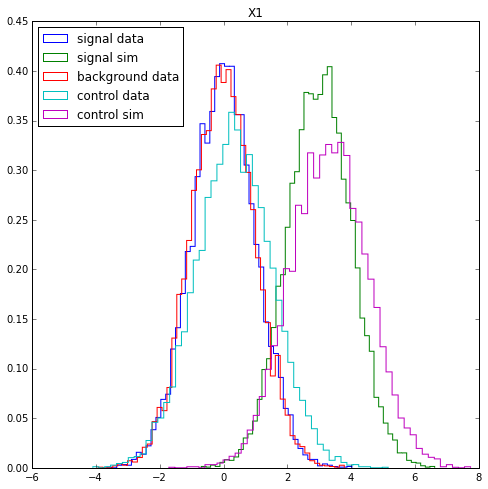
\includegraphics[width=0.6\textwidth]{x1.png}
\end{figure}

$X_1$ is irrelevant for distinguishing real data signal from real data
background but, because of simulation imperfections, has discriminative power
between simulated events and real data events.

\end{frame}

\begin{frame}

\begin{figure}
\centering
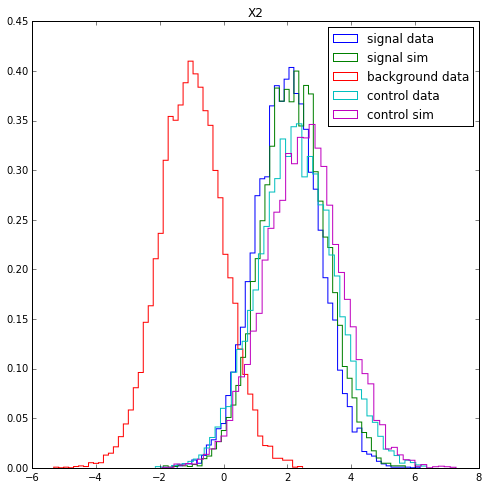
\includegraphics[width=0.6\textwidth]{x2.png}
\end{figure}

$X_2$ is discriminative between signal and background events.

\end{frame}

\begin{frame}

\begin{figure}
\centering
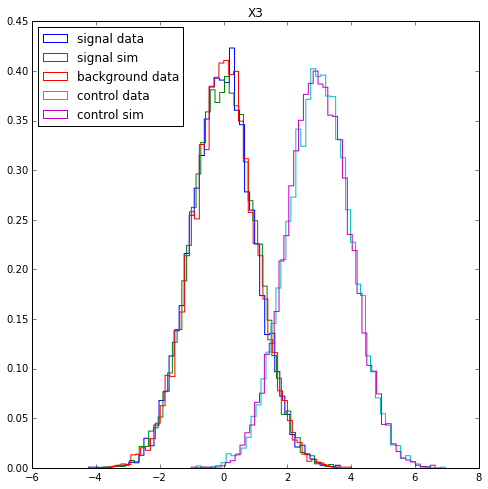
\includegraphics[width=0.6\textwidth]{x3.png}
\end{figure}

$X_3$ is discriminative between events from the original problem and the
control channel, but has otherwise no discriminative power between signal and
background events.

\end{frame}

\begin{frame}[fragile]
  \frametitle{Random exploration}

{\scriptsize
\begin{pythoncode}
from sklearn.ensemble import ExtraTreesClassifier

def find_best_tree(X_train, y_train, X_test, y_test,
                   X_data, y_data, X_control_sim, X_control_data):
    best_auc_test, best_auc_data = 0, 0
    best_ks = 0
    best_tree = None

    for seed in range(2000):
        clf = ExtraTreesClassifier(n_estimators=1, max_features=1,
                                   max_leaf_nodes=5, random_state=seed)
        clf.fit(X_train, y_train)
        auc_test = roc_auc_score(y_test, clf.predict_proba(X_test)[:, 1])
        auc_data = roc_auc_score(y_data, clf.predict_proba(X_data)[:, 1])
        ks = ks_statistic(clf.predict_proba(X_control_sim)[:, 1],
                          clf.predict_proba(X_control_data)[:, 1])

        if auc_test > best_auc_test and ks < 0.09:
            best_auc_test = auc_test
            best_auc_data = auc_data
            best_ks = ks
            best_tree = clf

    return best_auc_test, best_auc_data, best_ks, best_tree
\end{pythoncode}
}

\end{frame}

\begin{frame}[fragile]
  \frametitle{Random exploration}

{\scriptsize
\begin{pythoncode}
auc_test, auc_data, ks, tree = find_best_tree(X_train, y_train,
                                              X_test, y_test,
                                              X_data, y_data,
                                              X_control_sim, X_control_data)

print "ROC AUC (simulated signal vs. data background) =", auc_test
print "ROC AUC (data signal vs. data background) =", auc_data
print "KS statistic =", ks

>>> ROC AUC (simulated signal vs. data background) = 0.986357983199
>>> ROC AUC (data signal vs. data background) = 0.90973817
>>> KS statistic = 0.0578
\end{pythoncode}
}

\end{frame}

\begin{frame}
What just happened? By chance, we have found a classifier that
\begin{itemize}
\item has seemingly good test performance (AUC=0.986 on simulated signal versus real data background); and
\item passes the control channel test that we have defined.
\end{itemize}
{\color{blue} This classifier appears to be exactly the one we were seeking}.
\vspace{1cm}

{\color{red}Wrong}. The expected ROC AUC of 0.91 on real data signal and real data
background is significantly lower than our first estimate, suggesting that
there is still something wrong.

\end{frame}

\begin{frame}
\begin{figure}
\centering
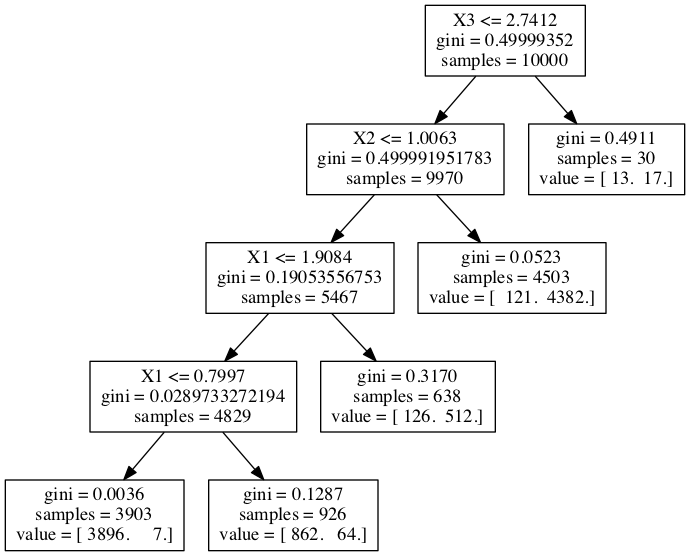
\includegraphics[width=0.7\textwidth]{tree.png}
\end{figure}

$\varphi$ exploits $X_1$, i.e. simulation versus real data
artefacts to indirectly classify signal from background events, {\color{red}while still passing the
control channel test} because of its use of $X_3$!

\end{frame}


\begin{frame}
  \frametitle{Winning the challenge}

As in the challege, simulation versus real data patterns may be hidden into
several variables, making it not possible to detect the problem by eye by
looking at variables individually. However, a learning algorithm might still be
able to exploit them, either by chance or on purpose.

\vspace{0.5cm}

Recipe for winning the challenge:
\begin{enumerate}
\item learn to distinguish between training and control data,
\item build a classifier on training data, with all the freedom to exploit simulation artefacts,
\item assign random predictions to samples predicted as control data, otherwise predict using the classifier found in the previous step.
\end{enumerate}

\end{frame}

\begin{frame}
  \frametitle{A better protocol}

If differences between simulated and real data events are fixed, then the
problem goes away.

\vspace{1cm}

One way to do it is to {\color{blue} learn a transformation (e.g., a reweighting) from
simulation onto real data from the control channel}, and then learn on
transformed simulated signal events versus real data background events.

\end{frame}



\end{document}
